\documentclass[12pt]{article}

\usepackage{booktabs}
\usepackage{tabularx}
\usepackage{longtable}
\usepackage{hyperref}
\usepackage{graphicx}
\usepackage[center]{caption}
\usepackage{float}
\captionsetup{justification=centering}

\hypersetup{ bookmarks=true,         % show bookmarks bar?
    colorlinks=true,      % false: boxed links; true: colored links
    linkcolor=red,          % color of internal links (change box color with
    citecolor=green,        % color of links to bibliography
    filecolor=magenta,      % color of file links
    urlcolor=cyan           % color of external links
}

\newcommand{\lips}{\textit{Insert your content here.}}
%% Comments

\usepackage{color}

\newif\ifcomments\commentstrue %displays comments
%\newif\ifcomments\commentsfalse %so that comments do not display

\ifcomments
\newcommand{\authornote}[3]{\textcolor{#1}{[#3 ---#2]}}
\newcommand{\todo}[1]{\textcolor{red}{[TODO: #1]}}
\else
\newcommand{\authornote}[3]{}
\newcommand{\todo}[1]{}
\fi

\newcommand{\wss}[1]{\authornote{blue}{SS}{#1}} 
\newcommand{\plt}[1]{\authornote{magenta}{TPLT}{#1}} %For explanation of the template
\newcommand{\an}[1]{\authornote{cyan}{Author}{#1}}

%% Common Parts

\newcommand{\progname}{Software Engineering} % PUT YOUR PROGRAM NAME HERE
\newcommand{\authname}{Team 21, Alkalytics
\\ Sumanya Gulati - gulats10
\\ Kate Min - mink9
\\ Jennifer Ye - yej52
\\ Jason Tran - tranj78} % AUTHOR NAMES                  

\usepackage{hyperref}
    \hypersetup{colorlinks=true, linkcolor=blue, citecolor=blue, filecolor=blue,
                urlcolor=blue, unicode=false}
    \urlstyle{same}
                                


\title{User Guide for \progname: Alkalytics} 
\author{\authname}
\date{\today}

\begin{document}

\maketitle
\newpage
\tableofcontents
\newpage

\section{Introduction}
\subsection*{Section Overview}
This section provides an orientation to the Alkalytics application, its purpose,
and the scope of this documentation.

Welcome to the Alkalytics User Guide. This comprehensive document provides
complete instructions for installing, configuring, and using all features of the
Alkalytics web application.

\subsection{Purpose}
Alkalytics is designed to:
\begin{itemize}
\item Manage experimental data efficiently
\item Provide powerful analysis tools
\item Generate customizable visualizations
\item Support collaborative research workflows
\end{itemize}

\section{System Overview}
\subsection*{Section Overview}
This section describes the technical architecture, components, and requirements
for running Alkalytics.

\subsection{Architecture}
Alkalytics is a React and TypeScript-based web application that runs locally for
security purposes. The system architecture consists of:

\begin{itemize}
\item \textbf{Frontend}: Built with React and TypeScript
\item \textbf{Backend}: Python processing with Univcorn server
\item \textbf{Database}: MongoDB for data storage
\end{itemize}

\subsection{Detailed Requirements}
\subsubsection*{Description}
Lists all hardware and software requirements for running the application.

\subsubsection{Hardware Requirements}
\begin{table}[H]
    \centering
    \begin{tabularx}{\textwidth}{llX}
        \toprule
        \textbf{Component} & \textbf{Minimum} & \textbf{Recommended} \\
        \midrule
        RAM & 8GB & 16GB \\
        Storage & 10GB & 50GB SSD \\
        Processor & 2 cores & 4 cores \\
        \bottomrule
    \end{tabularx}
\end{table}

\subsubsection{Software Dependencies}
\begin{table}[H]
    \centering
    \begin{tabularx}{\textwidth}{lXl}
        \toprule
        \textbf{Software} & \textbf{Purpose} & \textbf{Version} \\
        \midrule
        Node.js & Frontend runtime & 16.x LTS \\
        MongoDB & Database & 5.0+ \\
        Python & Backend processing & 3.8+ \\
        Univcorn & ASGI server & 0.15+ \\
        \bottomrule
    \end{tabularx}
\end{table}

\section{Installation Guide}
\subsection*{Section Overview}
This section provides complete step-by-step instructions for setting up the
Alkalytics environment.

\subsection{Step-by-Step Installation}
\begin{enumerate}
    \item \textbf{Prerequisite Installation}
    \begin{enumerate}
        \item Install Node.js from \url{https://nodejs.org}
        \item Install MongoDB from \url{https://www.mongodb.com}
        \item Install Python 3.x from \url{https://www.python.org}
    \end{enumerate}
    
    \item \textbf{Repository Setup}
    \begin{verbatim}
    git clone https://github.com/your-repo/alkalytics.git
    cd alkalytics
    \end{verbatim}
    
    \item \textbf{Dependency Installation}
    \begin{verbatim}
    yarn install
    pip install -r requirements.txt
    \end{verbatim}
    
    \item \textbf{Database Configuration}
    \begin{enumerate}
        \item Create data directory:
        \begin{verbatim}
        mkdir /data/db
        \end{verbatim}
        \item Start MongoDB service:
        \begin{verbatim}
        mongod --dbpath /data/db --port 27017
        \end{verbatim}
    \end{enumerate}
    
    \item \textbf{Application Launch}
    \begin{enumerate}
        \item Start backend:
        \begin{verbatim}
        yarn ts-node src/utils/server.ts
        \end{verbatim}
        \item Start frontend:
        \begin{verbatim}
        yarn start
        \end{verbatim}
        \item Launch ASGI server:
        \begin{verbatim}
        univcorn --port 8000 main:app
        \end{verbatim}
    \end{enumerate}
\end{enumerate}

\subsection{Verification}
After installation, verify all components are running:
\begin{enumerate}
    \item Frontend: \texttt{http://localhost:3000}
    \item Backend: \texttt{http://localhost:8000/healthcheck}
    \item Database: Check MongoDB connection on port 27017
\end{enumerate}

\section{User Management}
\subsection*{Section Overview}
This application has different user roles. Each role has a different set of
permissions and respective capabilities within the application.

\subsection{Admin and Researcher Role}
Administrators have full control over all system functionality including data
management, user configuration, and system settings. Both Admin and Researcher
roles have the same permissions. \newline \newline
These features include:
\begin{itemize}
    \item Editing tables, including modifying cells, adding/removing rows and columns.
    \item Setting data types for columns.
    \item Using the Excel function bar for calculations.
    \item Computing efficiency metrics.
    \item Managing bulk data uploads.
    \item Generating and exporting graphs.
\end{itemize}

\subsection{Researcher Assistant Role}
Researcher assistants can view data, run analyses, and generate reports but have limited
system configuration capabilities. \newline\newline
These features include:
\begin{itemize}
    \item Viewing and searching tables (Experiment, Efficiency, and Raw Data).
    \item Searching within a specific column or the entire table.
    \item Generating graphs but with restricted data modification capabilities.
\end{itemize}

\newpage
\section{Web Application Pages}
\subsection*{Section Overview}
This section covers all data handling operations including uploads, processing,
and table management.

\subsection{Login and Sign Up Process}
When users first load onto the page, they will be greated by a log in screen. 
If the user has login credentions, log in as normal 
\begin{figure}[H]
    \centering
    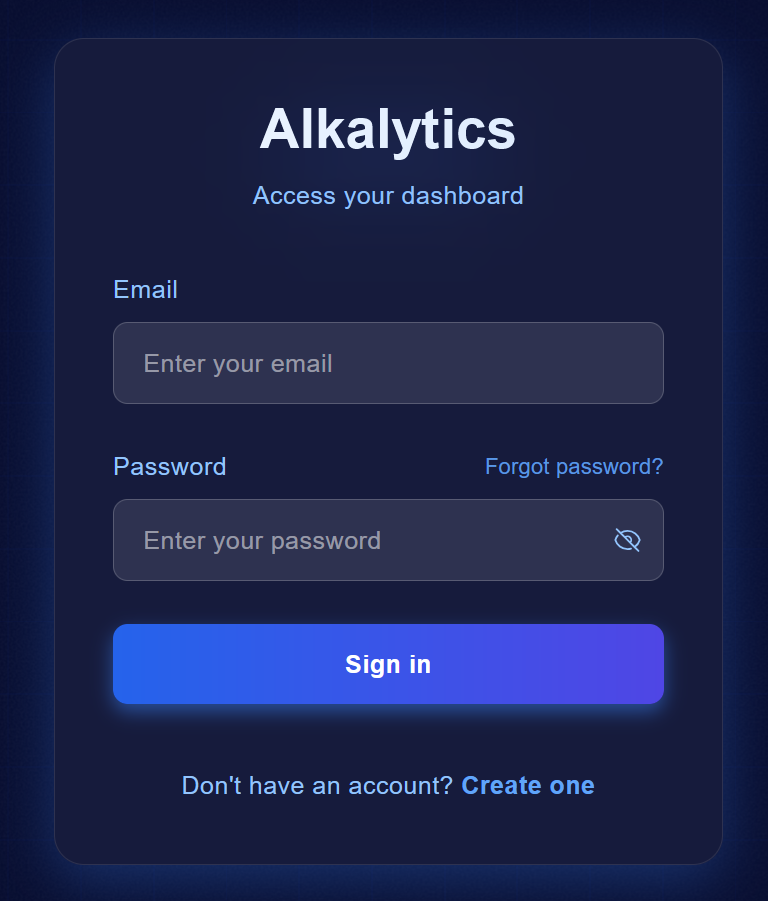
\includegraphics[scale=0.55]{Images/login .png}
    \caption{Login Form}
    \label{fig:example}
\end{figure}

\subsection{Sign Up Process}
If users do not have an account, they will need to create one by clicking the
\textbf{Create one} button at the bottom of the login form. The user must then
enter an email and desired password. There will be three roles to pick from,
Admin, Researcher and Research Assistant. After creating a user account, log in
as normal. 
\begin{figure}[H]
    \centering
    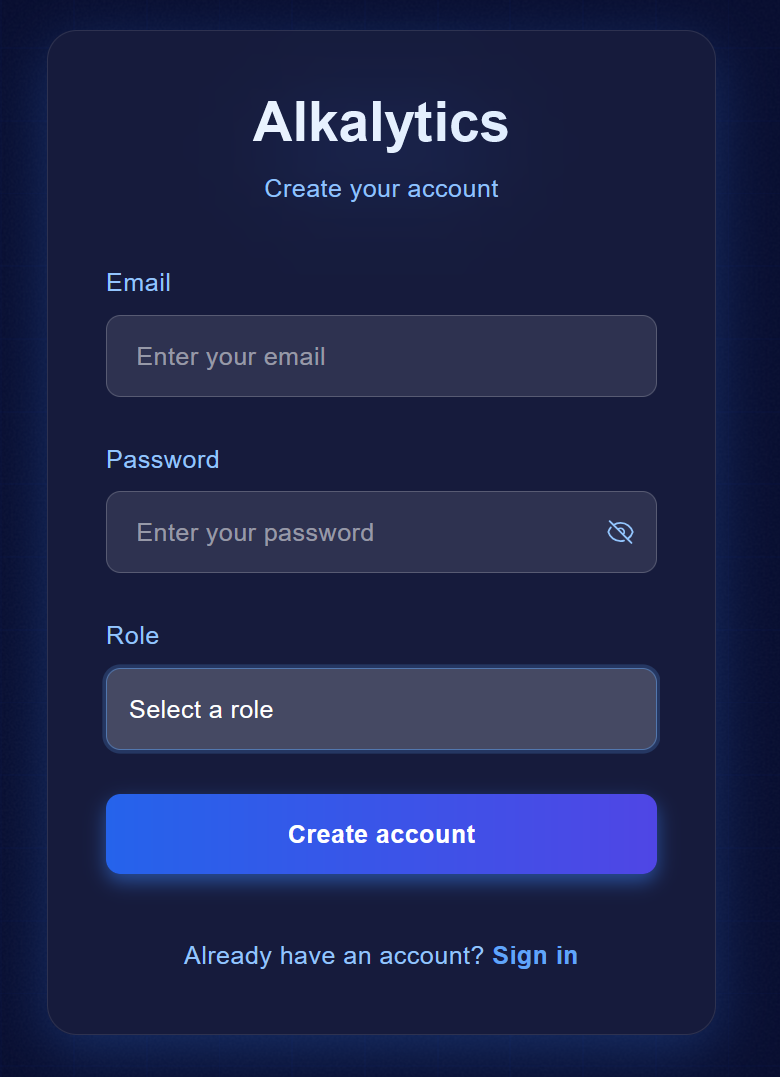
\includegraphics[scale=0.55]{Images/sign up .png}
    \caption{Sign Up Form}
    \label{fig:example}
\end{figure}

\subsection{Upload Process}
\subsubsection*{Description}
The upload functionality allows users to import experimental data in various
formats for analysis.

\subsubsection{Step-by-Step Upload}
\begin{enumerate}
    \item Navigate to Upload Page
    \item Select file type (Experiment Log or Raw Data)
    \item Choose upload method:
    \begin{itemize}
        \item Drag and drop files
        \item Browse file system
    \end{itemize}
    \item Verify file preview
    \item Click \textbf{Upload} button
    \item Monitor progress in notification panel
\end{enumerate}

\subsubsection{File Requirements}
\begin{table}[H]
    \centering
    \begin{tabularx}{\textwidth}{lX}
        \toprule
        \textbf{Requirement} & \textbf{Specification} \\
        \midrule
        File Size & Maximum 10MB per file \\
        Columns & Minimum 5 required fields \\
        Date Format & YYYY-MM-DD \\
        Special Characters & Avoid in header names \\
        \bottomrule
    \end{tabularx}
\end{table}

\subsection{Table View}

\subsubsection{Table Editing}
\begin{enumerate}
    \item Navigate to Experiment Table
    \item Click \textbf{Edit} button to enable editing mode
    \item Modify cell values directly
    \item Use \textbf{Save} button to commit changes
\end{enumerate}

\subsubsection{Column Management}
\begin{itemize}
    \item \textbf{Adding Columns:}
    \begin{enumerate}
        \item Click \textbf{Add Column} button
        \item Enter column name in dialog
        \item Select data type from dropdown
        \item Click \textbf{Add Column} to confirm
    \end{enumerate}
    
    \item \textbf{Removing Columns:}
    \begin{enumerate}
        \item Click \textbf{Remove Column} button
        \item Select column from dropdown
        \item Confirm deletion
    \end{enumerate}
\end{itemize}

\subsubsection{Excel Function Bar}
\begin{enumerate}
    \item Select target rows using checkboxes
    \item Choose destination column
    \item Enter formula (e.g., \texttt{SUM(A,B)})
    \item Click \textbf{Apply} to execute
\end{enumerate}

\subsection{Graph Generation}
\subsection*{Section Overview}
This section provides detailed instructions for creating, customizing, and
exporting data visualizations.

\subsection*{Page Overview}
The graph page is seperated in two sections. 
\newline \newline
\textbf{Side Bar:} \newline
On the left side of the page is the sidebar where it displays all the recently
generated graphs and has the generate new graph button.
\newline\newline

\noindent \textbf{Main Content:}\newline
On the right is the main content of the page. Here, the generated graph will be
displayed along with a quick linear regression analysis with a short statement
of its findings 
\begin{figure}[H]
    \centering
    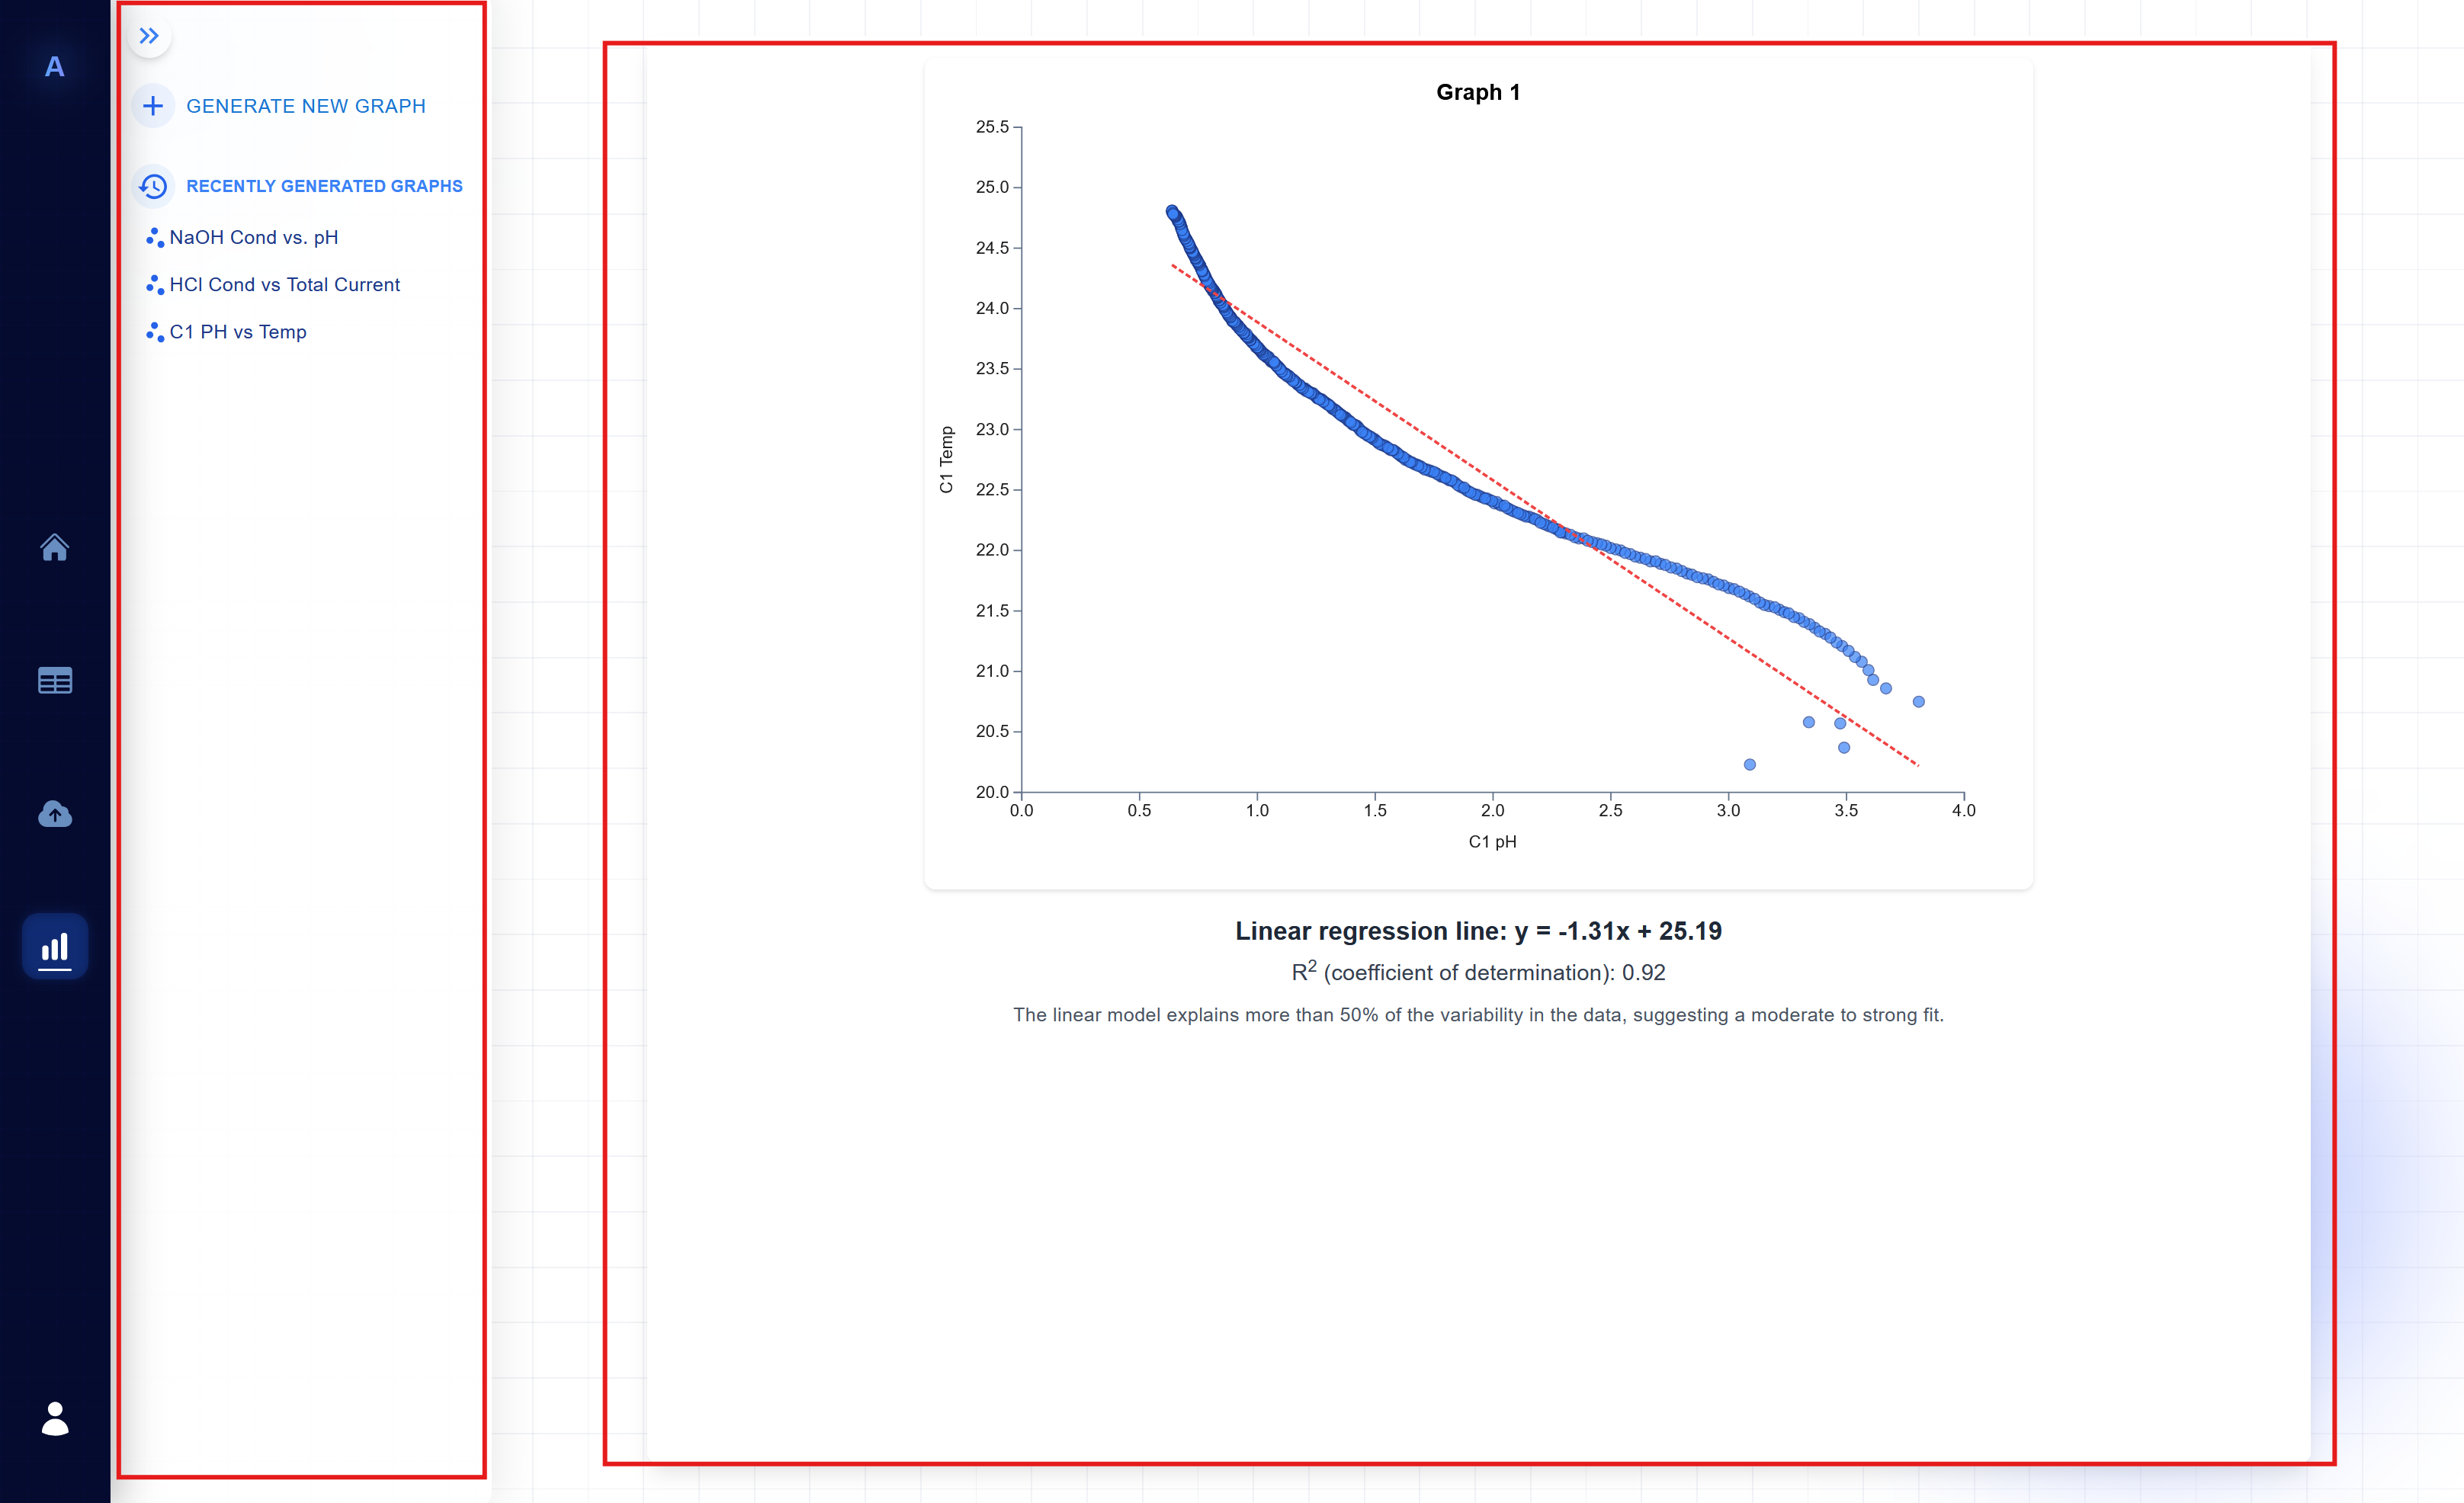
\includegraphics[scale=0.3]{Images/graph page .png}
    \caption{Graph page Seperation Display}
    \label{fig:example}
\end{figure}

On the side bar, beside each generated graph item has an icon which signifies
the type of graph it is. 
\begin{table}[H]
    \centering
    \begin{tabular}{|c|c|}
        \hline
         \textbf{Icon} & \textbf{Definition} \\
        \hline
        
\includegraphics[width=1.5cm]{Images/graph-line.png} & Line Graph \\
        \hline
        
\includegraphics[width=1.5cm]{Images/graph-bar.png} & Bar Graph \\
        \hline
        
\includegraphics[width=1.5cm]{Images/graph-scatter.png} & Scatter Plot \\
        \hline
    \end{tabular}
    \caption{Graph Types and Their Definitions}
    \label{tab:graphs}
\end{table}

\noindent \textbf{Generting a New Graph:} \newline
To create a new graph, click on the \textbf{Generate New Graph} button at the top of the side bar:
\begin{figure}[H]
    \centering
    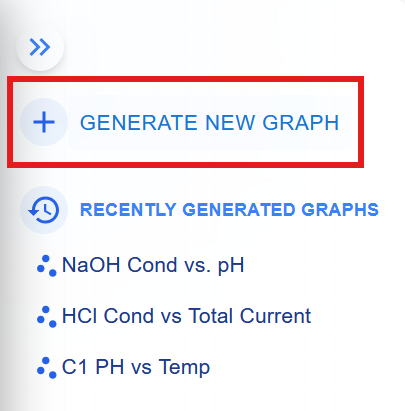
\includegraphics[scale=1]{Images/graph-newgraph .png}
    \caption{Highlights the Generate New Graph Button}
    \label{fig:example}
\end{figure}
\subsubsection{Detailed Workflow}
\subsubsection*{Description}
There is a five-step process for generating custom graphs from experimental data.

\begin{enumerate}
    \item \textbf{Select Graph Type:} \newline
    The app currently only supports 3 types of graphs. 
    \begin{itemize}
        \item Line graph 
        \item Bar graph 
        \item Scatter plot
    \end{itemize}
    \begin{figure}[H]
        \centering
        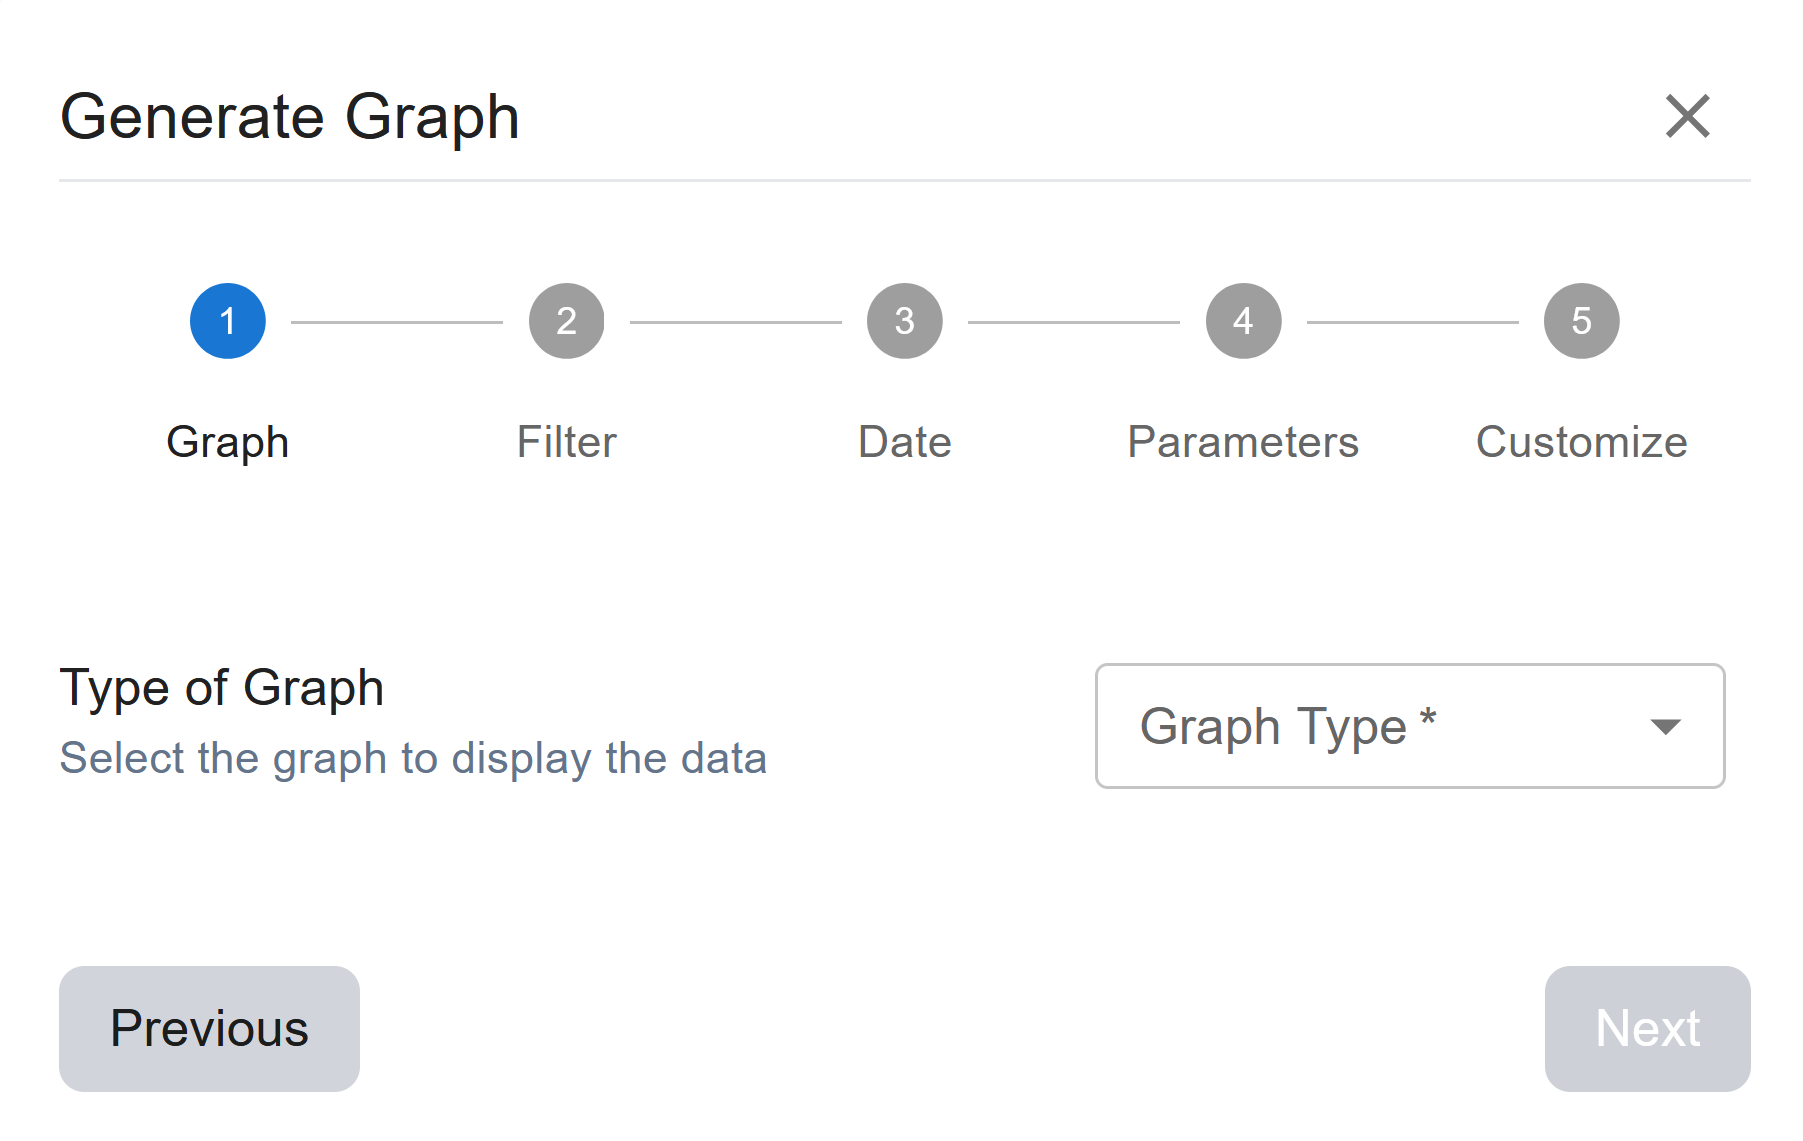
\includegraphics[scale=0.4]{Images/graph-form .png}
        \caption{Highlights the Generate New Graph Button}
        \label{fig:example}
    \end{figure}

    \item \textbf{Optional: Apply Filters}: \newline
    Use this part of the form to filter experiment dates based on a certain
    attribute. The attribute could be from the Experiment or Raw Data files.
    \newline
    \textbf{Note:} Either all form field must be willed out or all must be empty in order
    to progress to the next stage of the form. 
    \begin{enumerate}
        \item Choose which data file attribute to filter by
        \item Choose filter attribute 
        \item Select filter value from dropdown
    \end{enumerate}
    \begin{figure}[H]
        \centering
        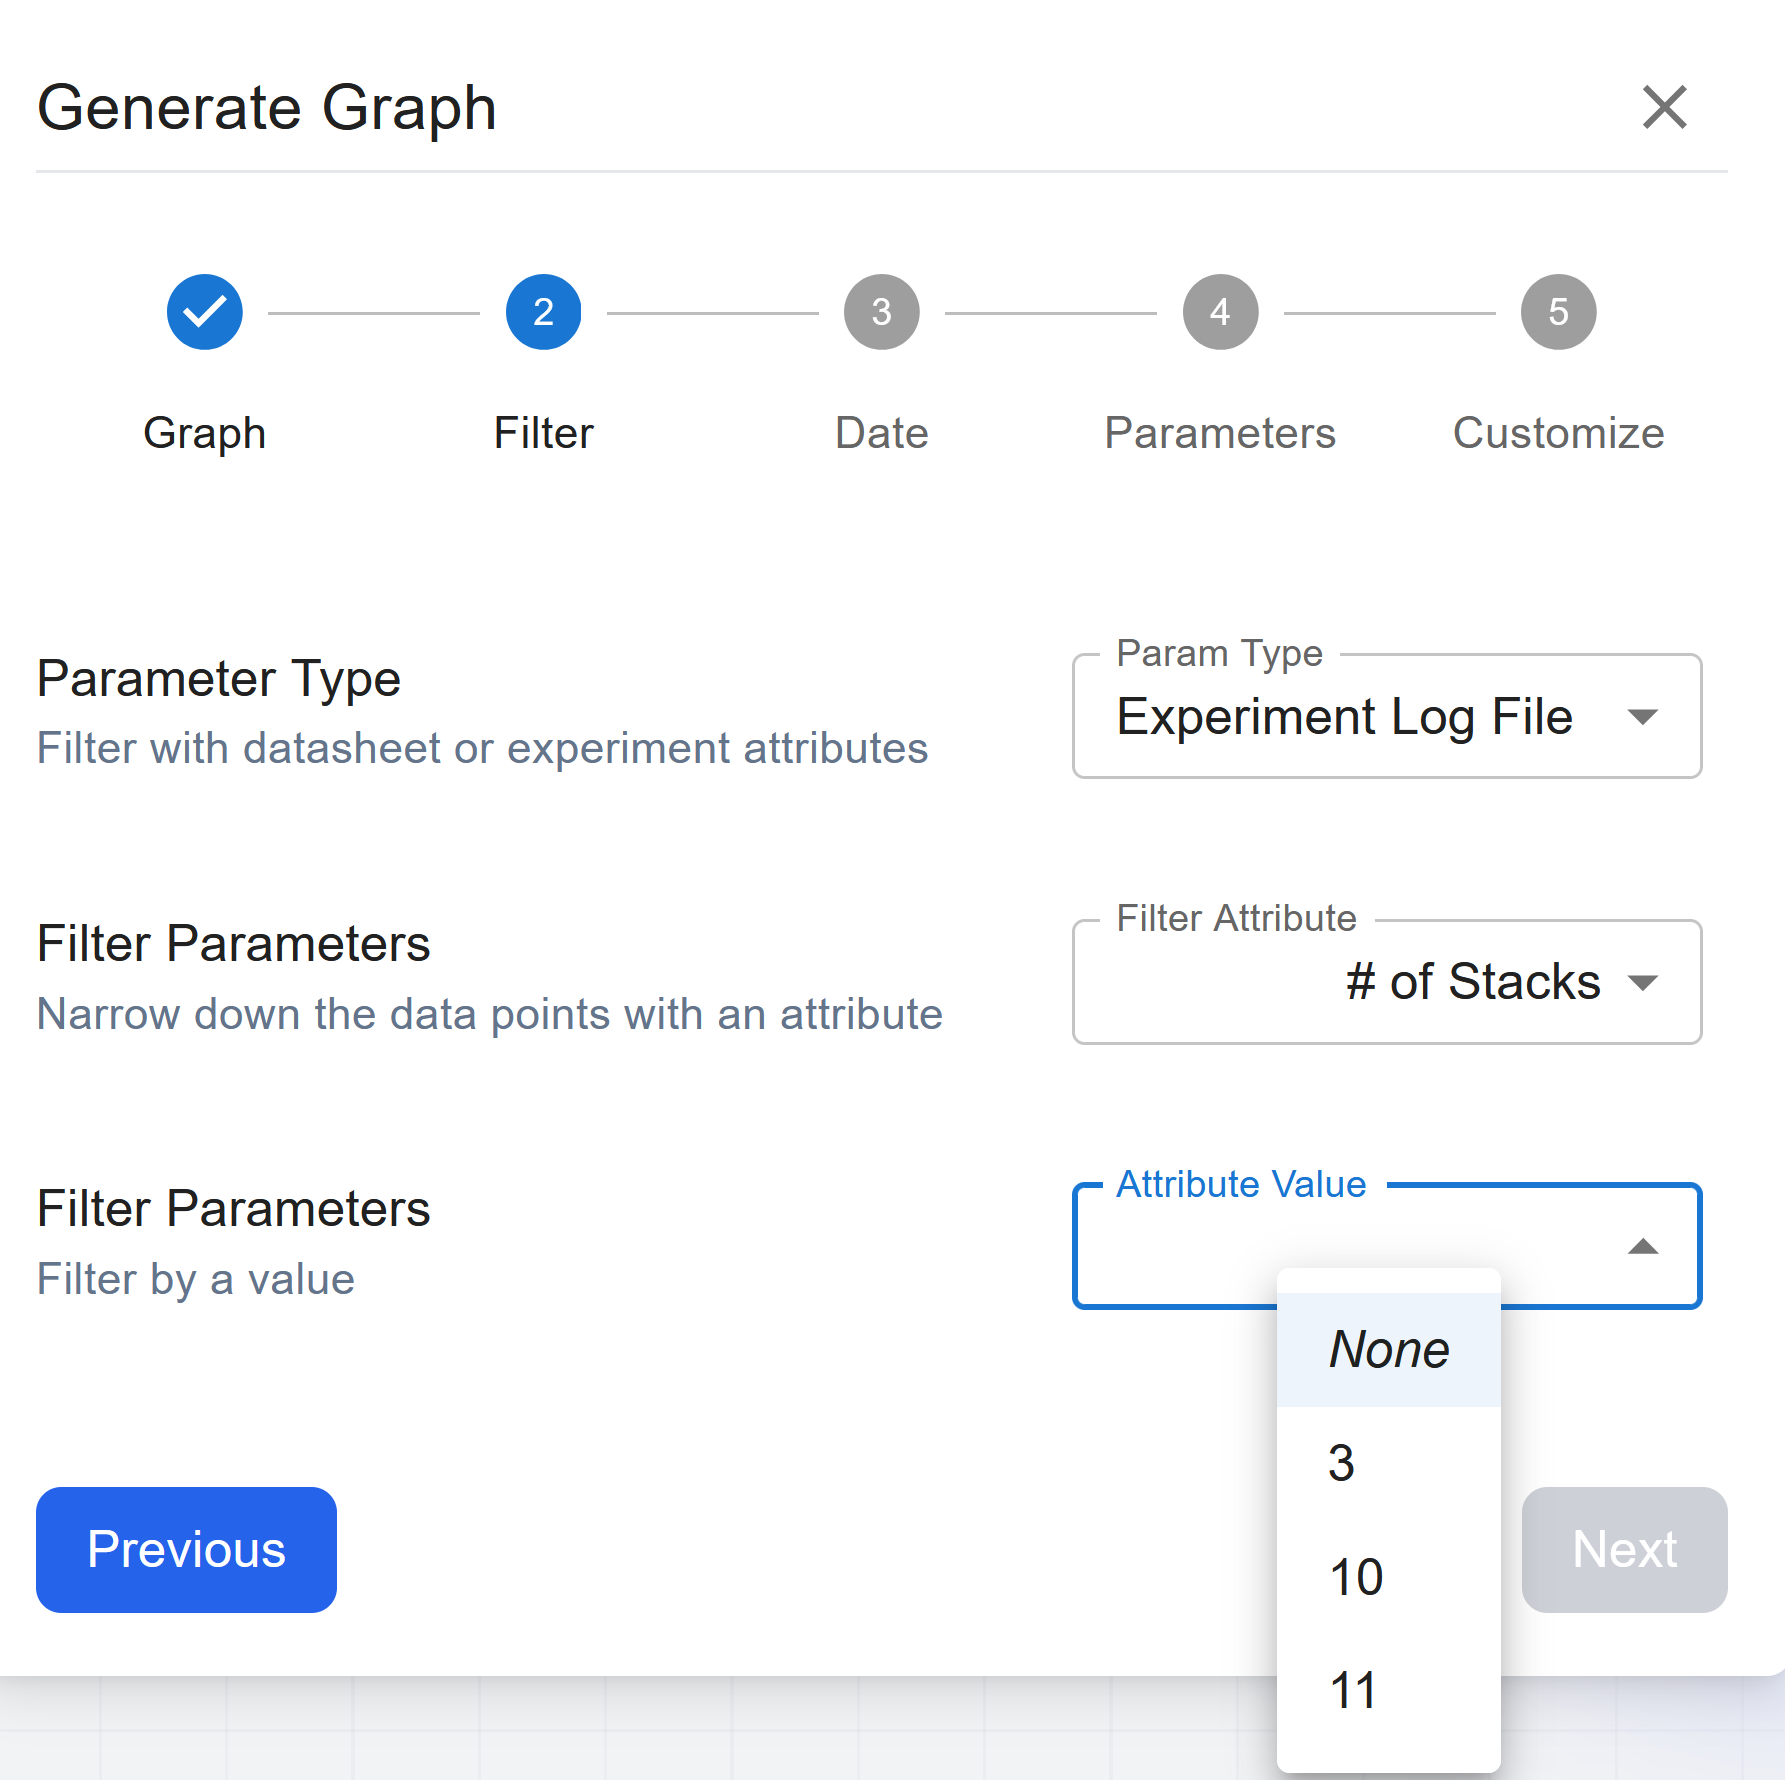
\includegraphics[scale=0.4]{Images/graph-filter.png}
        \caption{Sample Input of the Filter Step}
        \label{fig:example}
    \end{figure}

    \item \textbf{Selecting Dates}: \newline
    If no filter is applied, all experiemnt dates wil be listed. 
    \begin{figure}[H]
        \centering
        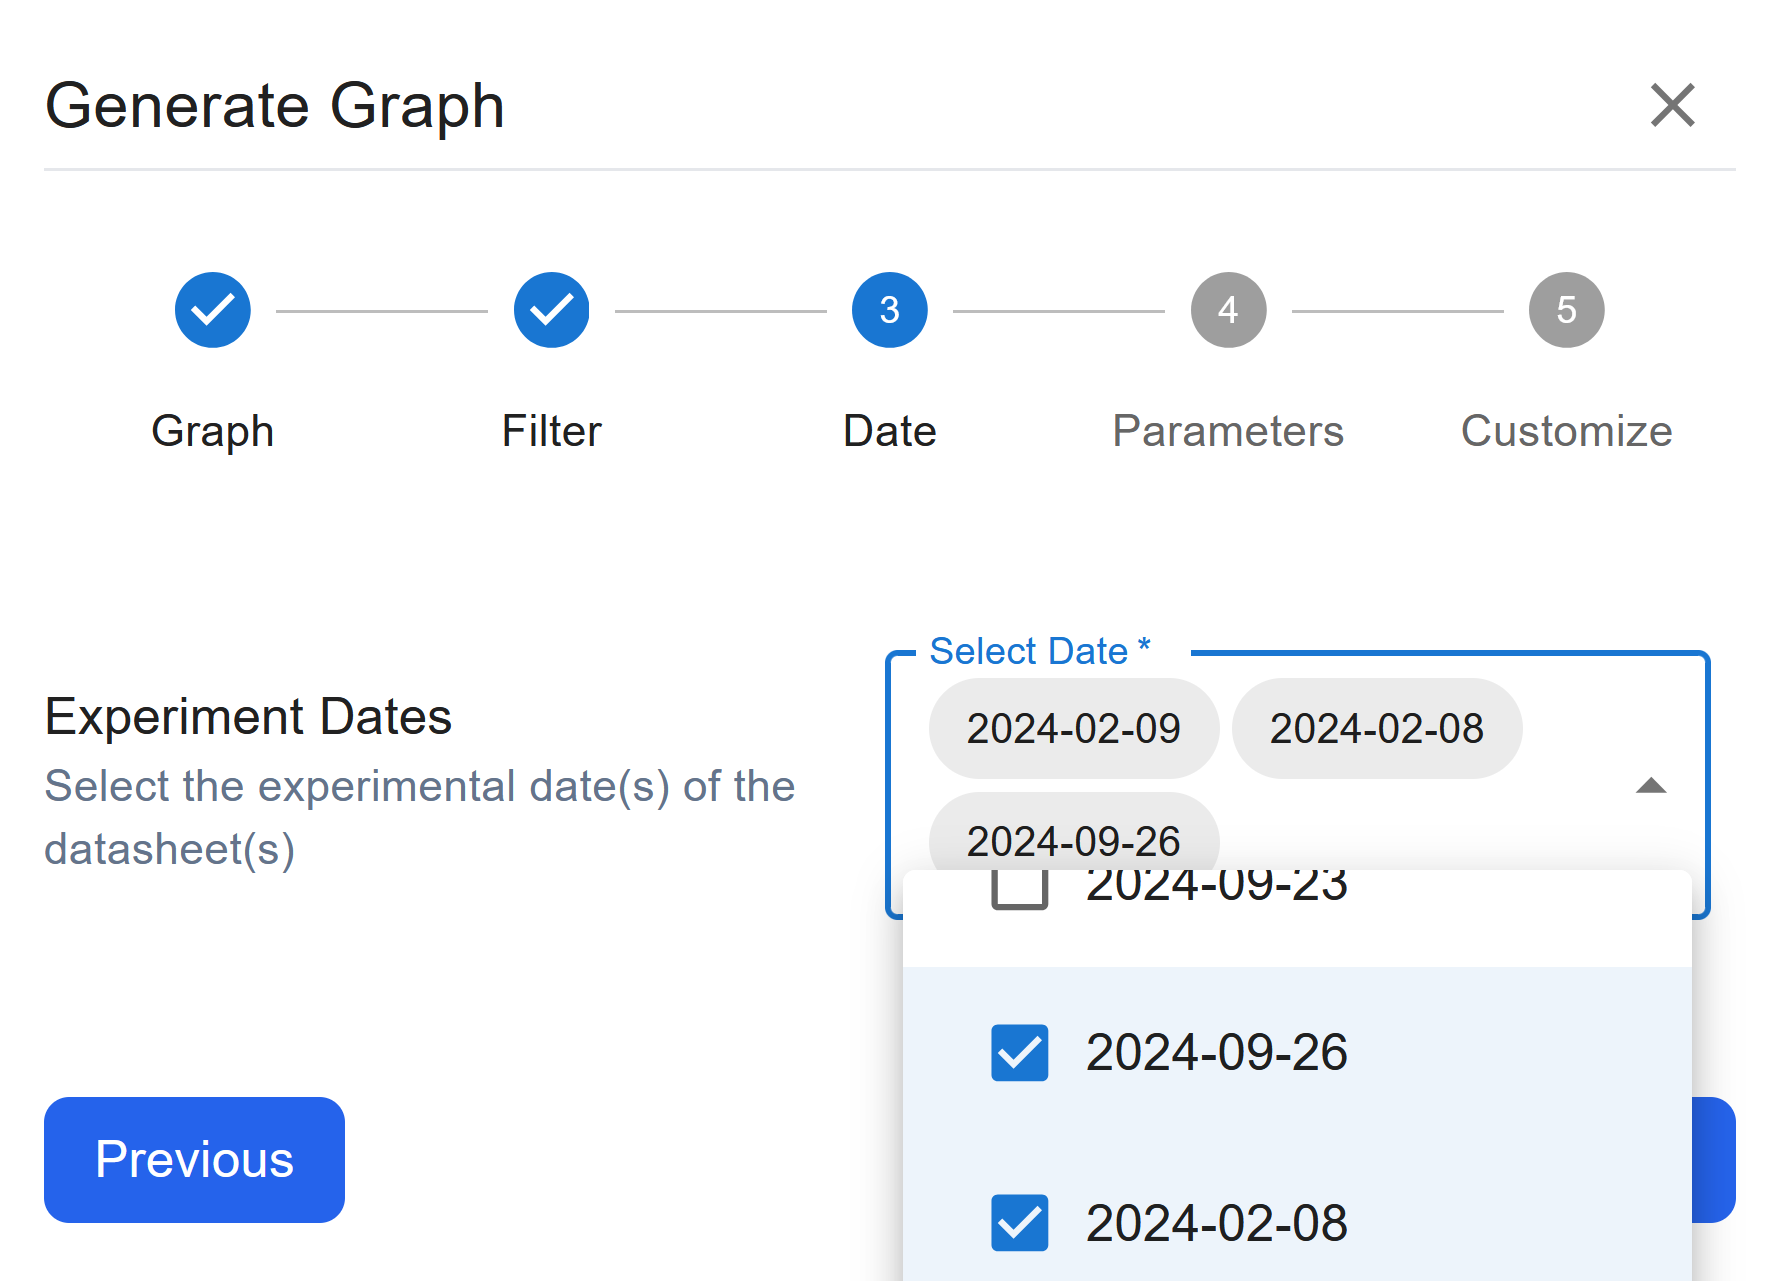
\includegraphics[scale=0.4]{Images/graph-dates.png}
        \caption{Sample Input of the Date Step}
        \label{fig:example}
    \end{figure}
    
    \item \textbf{Set Parameters}: \newline
    Select the attributes for the X and Y axis to plot. The two attributes must
    be from the same experiment sheet. 
    \begin{figure}[H]
        \centering
        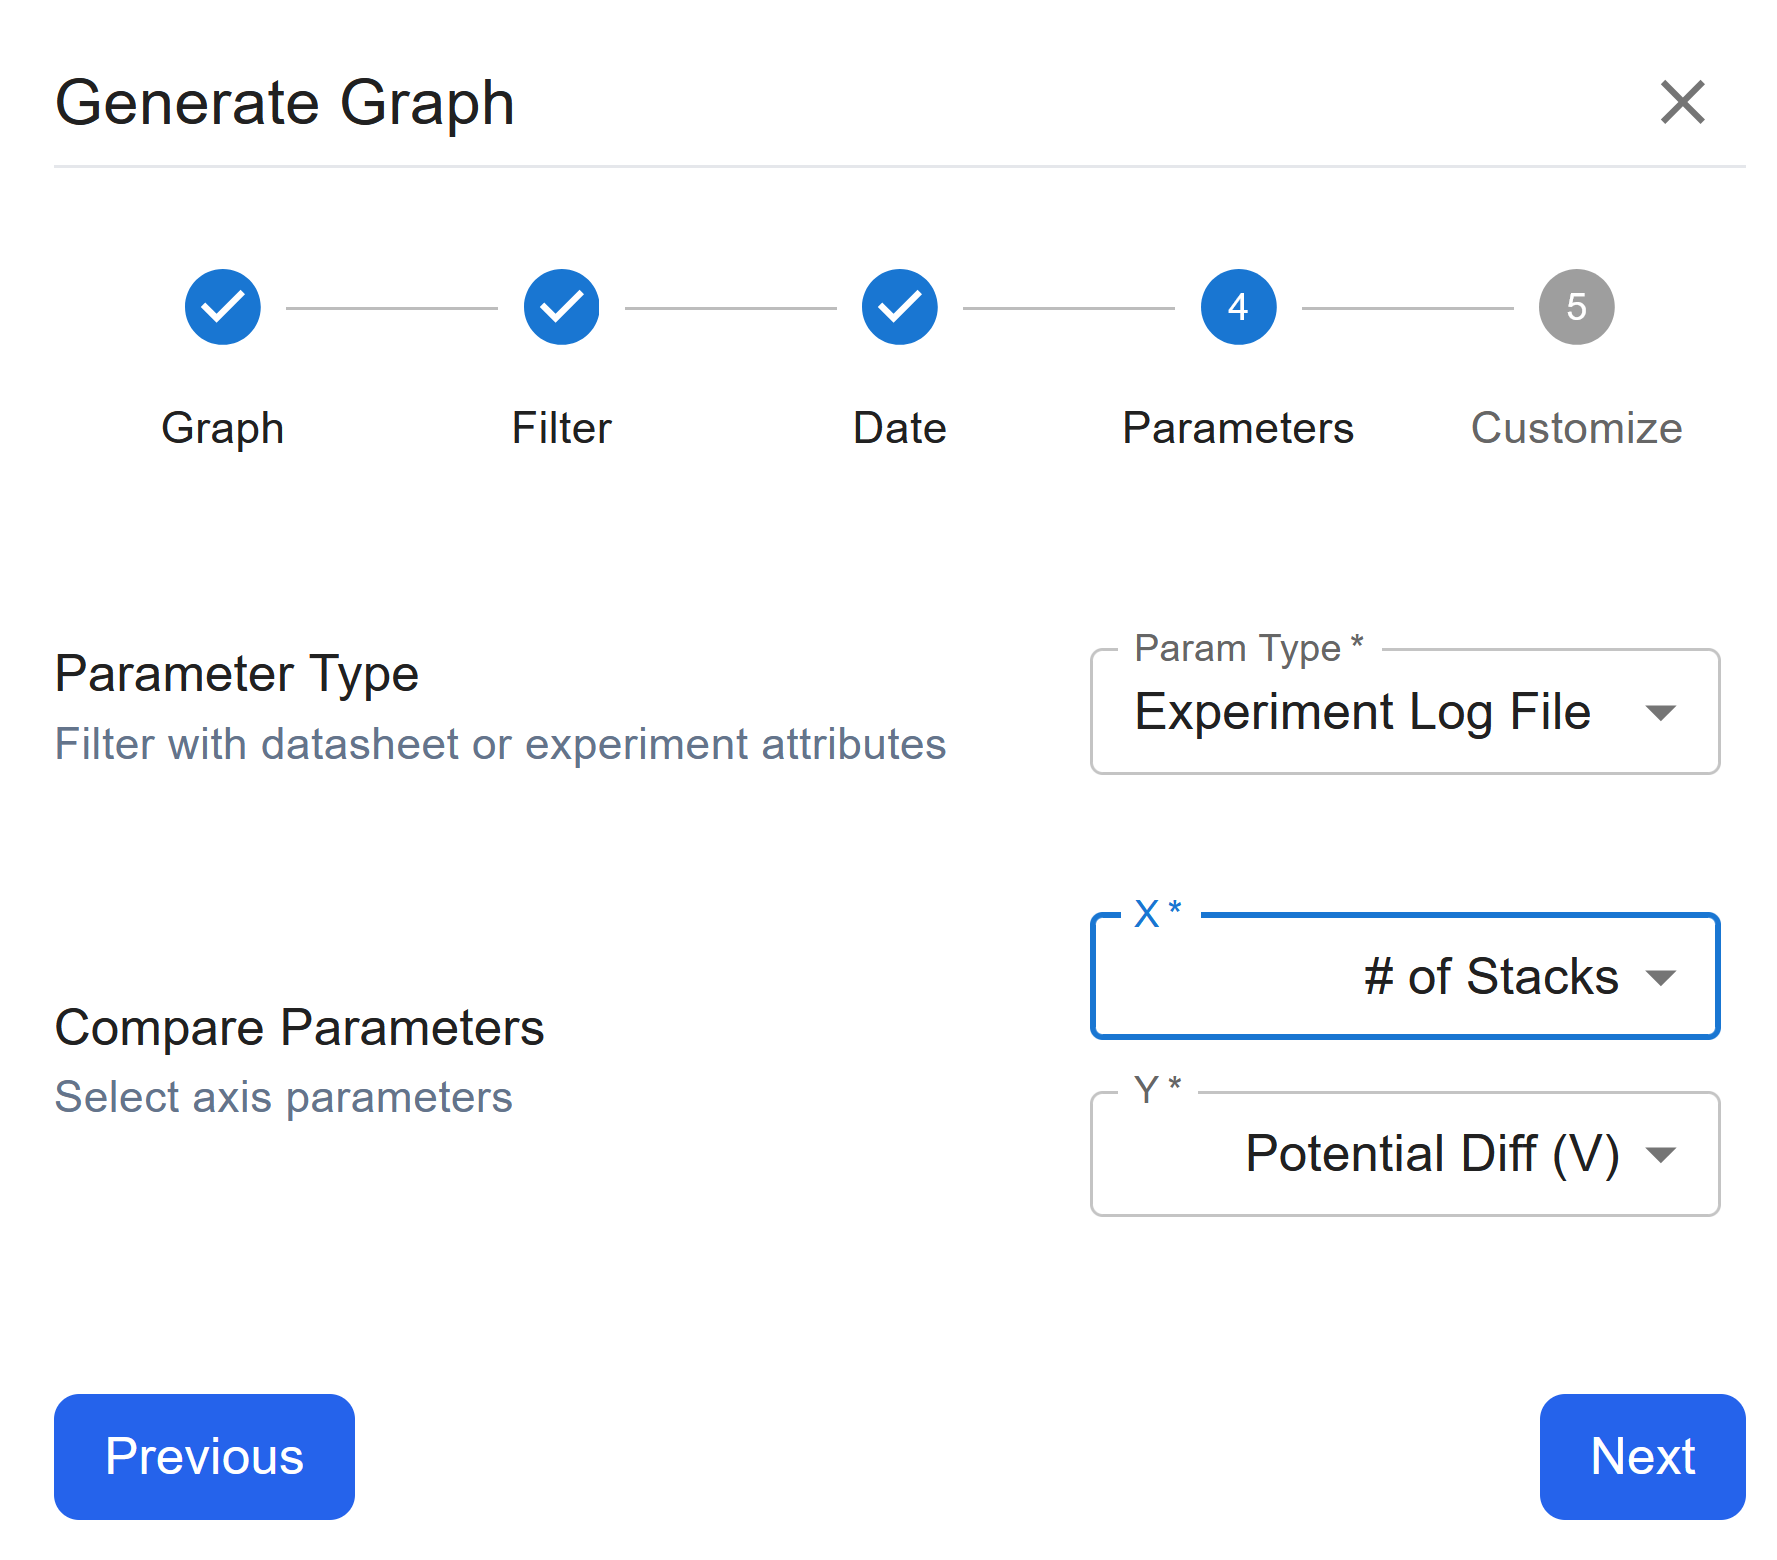
\includegraphics[scale=0.4]{Images/graph-param.png}
        \caption{Sample Input of the Filter Step}
        \label{fig:example}
    \end{figure}
    
    \item \textbf{Customize Display}: \newline
    Users are able to customize the graphs. All fields on this step are
    optional.If no axis labels are inputted, the axis would be nammed the
    attribute name selected by default.
    \newline
    There are the following options for customization
    \begin{itemize}
        \item Graph title
        \item Axis Ranges
        \item Axis Labels
    \end{itemize}
    \begin{figure}[H]
        \centering
        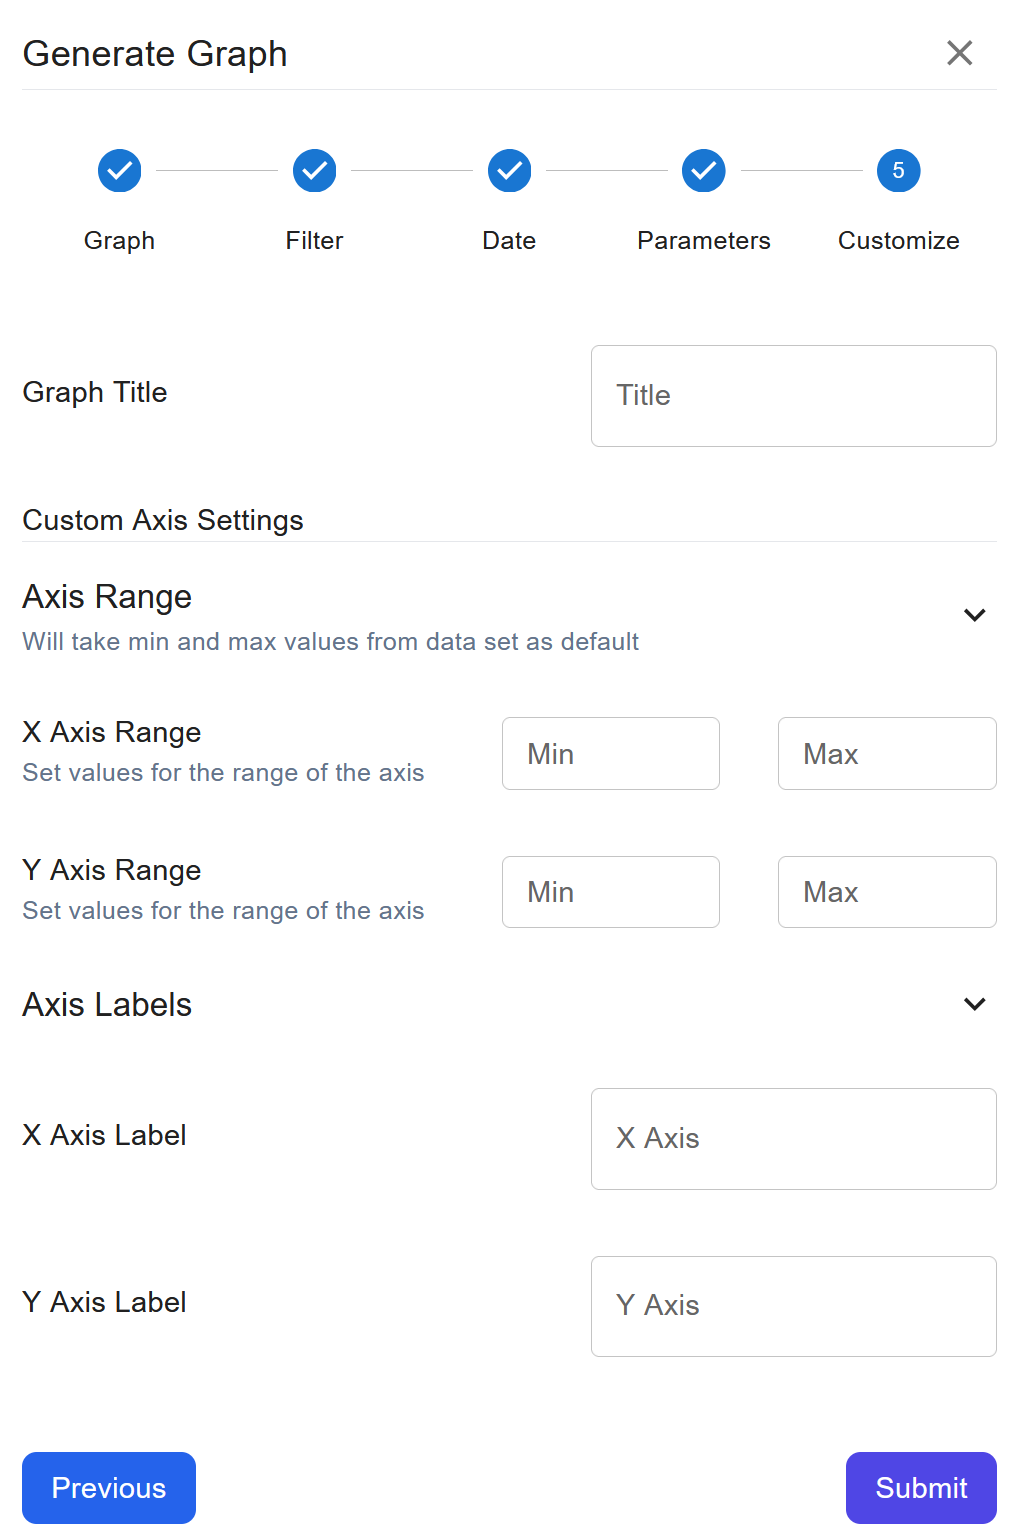
\includegraphics[scale=0.6]{Images/graph-custom.png}
        \caption{Sample Input of the Filter Step}
        \label{fig:example}
    \end{figure}
\end{enumerate}

\section{Troubleshooting}
\subsection*{Section Overview}
This section lists common issues, error messages, and their solutions, along
with advanced diagnostic procedures.

\subsection{Common Graphing Issues}

\begin{table}[H]
    \centering
    \begin{tabularx}{\textwidth}{lXl}
        \toprule
        \textbf{Issue} & \textbf{Solution} \\
        \midrule
        Dropdown options not appearing & There may be no value for the
        selected combination of attributes or filters. Check to verify inputted
        options \newline \\
        Frozen form & There may be a large number of options to select from.
        Please give the page a few minutes to finishing loading up and
        displaying all the data \newline \\
        Rendering failed & Validate data selection \\
        \bottomrule
    \end{tabularx}
\end{table}
\end{document}